\section{Simulations}
\label{S:experiments}%simple integrator example ???
In this section we shall control a single \sop\ continuous time plant
with $3$ \sop\ 'PID'-digital controllers, and $1$
system destabilizing-digital controller if it is not properly detected
and isolated.  The plant is described by the following equation:
\begin{equation*}
G_{\mathsf{pn}}(s) = \frac{k_{\mathsf{pn}}}{s+\omega_{\mathsf{pn}}} = \frac{2}{s+5},
\end{equation*}
The \sop\ 'PID'-digital controllers are of the following form:
\begin{equation*}
G_{\textsf{PID}}(z)=k_{\textsf{P}} + G_{\textsf{I}}(z)  + G_{\textsf{D}}(z)
\end{equation*}
in which $k_{\textsf{P}} > 0$ is the proportional term,
$G_{\textsf{I}}(z)$ is the 'integral' term which is synthesized by
applying the \IPESH{\it-transform}
\cite[Definition~4]{kottenstette09:_digit_contr_of_multip_discr} to
the following continuous-time 'integrator' model (N.B. this is an
integrator with finite-gain, such as seen when using a
lag-compensator, in which $\epsilon > 0$ can be arbitrarily small in
order to satisfy our \sop\ condition on the controller)
\begin{equation*}
G_{\textsf{I}}(s)=\frac{k_{\textsf{I}}}{s + \epsilon k_{\textsf{I}}}.
\end{equation*}
Similarly, $G_{\textsf{D}}(z)$ is the 'derivative' term which is
synthesized by applying the \IPESH{\it-transform} to the following
continuous-time 'derivative' model 
\begin{equation*}
G_{\textsf{D}}(s)=k_{\textsf{D}}\frac{\frac{NT_s}{\pi}s+1}{\frac{T_s}{\pi}s + 1}.
\end{equation*}
Note that $N > 1$, is typically chosen to be around $10$.
With our nominal plant given, we use the following loop-shaping
formulas to select the control gains in terms of the nyquist frequency
$\omega_{\mathsf{nyquist}} = \frac{\pi}{T_s}$.
\begin{gather*}
k_{\textsf{P}}=\alpha \frac{1}{3}\frac{\omega_{\mathsf{nyquist}} +
  \omega_{\mathsf{pn}}}{k_{\mathsf{pn}}},\ 
k_{\textsf{I}}=\alpha \frac{1}{3}\frac{\omega_{\mathsf{nyquist}}(\omega_{\mathsf{nyquist}} +
  \omega_{\mathsf{pn}})}{k_{\mathsf{pn}}}\\
k_{\textsf{D}}=\alpha \frac{1}{3}\frac{2}{1+N}\frac{\omega_{\mathsf{nyquist}} +
  \omega_{\mathsf{pn}}}{k_{\mathsf{pn}}}.
\end{gather*}
Other relevant parameters to the simulation are $b = 2,$ $T_s = .1,$ $\alpha =
1,$ $\epsilon = .001,$ $N=10$.  The unstable controller consisted of
the discrete-time version of the {\em negative} 'PID'-digital controller
with the integrator replaced with {\em three}-integrators.

Fig.~\ref{fig:fault_detection_off_nominal} shows the nominal system
response when all controllers are redundant, as we can see, the
controller is able to reject periodic step-like disturbances.
Fig.~\ref{fig:fault_detection_off_degrade} shows the effect when one
of the controllers is corrupted in a passive manner and looses its
integrator-term, when controllers loose the proportional-term the
overall degradation in performance is barely noticeable.
Fig.~\ref{fig:fault_detection_off_denial} shows that intermittent 
denial-of-service attacks lead to a graceful degradation and recovery
of performance as a single controller is being attacked on the
network.  We should note that the denial of service attack can also
be thought of as a single controller setting its integral,
proportional term and derivative term to zero.
Fig.~\ref{fig:fault_detection_off} shows that in a very short
period of time, the introduction of the destabilizing controller with
non-redundant-controller-detection disabled, system instability will
occur.  Fig~\ref{fig:fault_detection_on} indicates 
that when non-redundant-controller-detection is enabled the
destabilizing-controller is isolated from the rest of the network and
not only is stability preserved, but disturbances from
$r_{\mathsf{pn}}(t)$ are still eliminated.
\begin{figure}
  \centering
  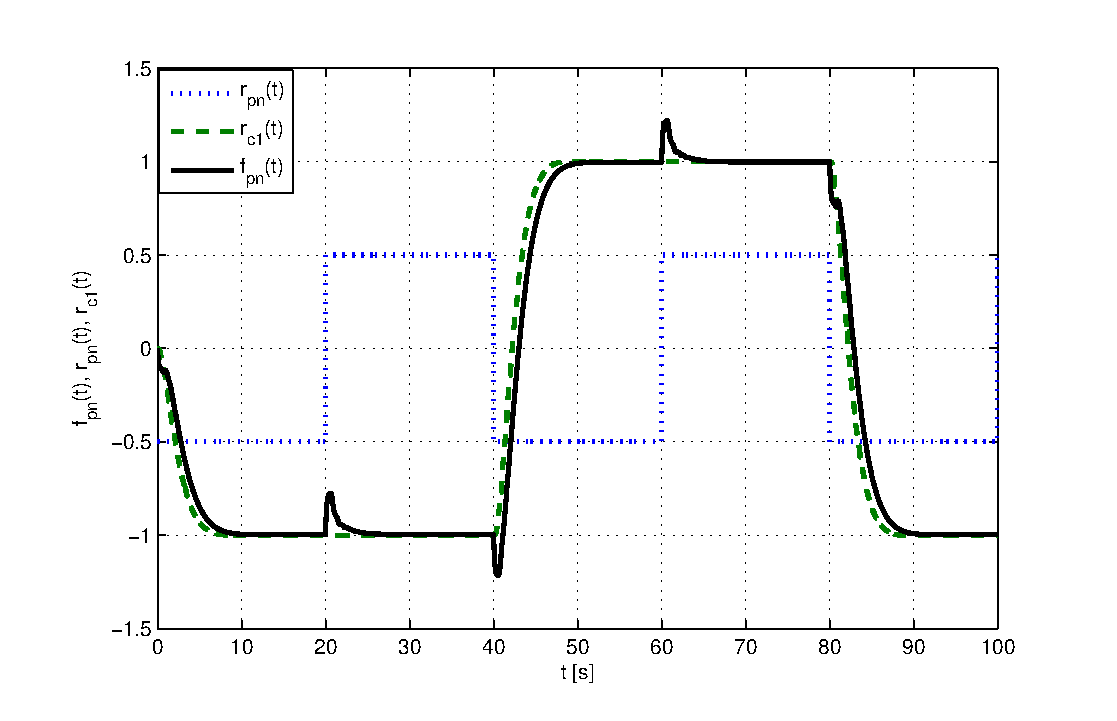
\includegraphics[width=3.5in]{figures/fault_detection_off_nominal}
  \caption{Nominal system response when using the {\em resilient power
    junction} under Assumption~\ref{A:resilient_pj} $\mathsf{m_c}=\mathsf{m}$.}
  \label{fig:fault_detection_off_nominal}
\end{figure}
\begin{figure}
  \centering
  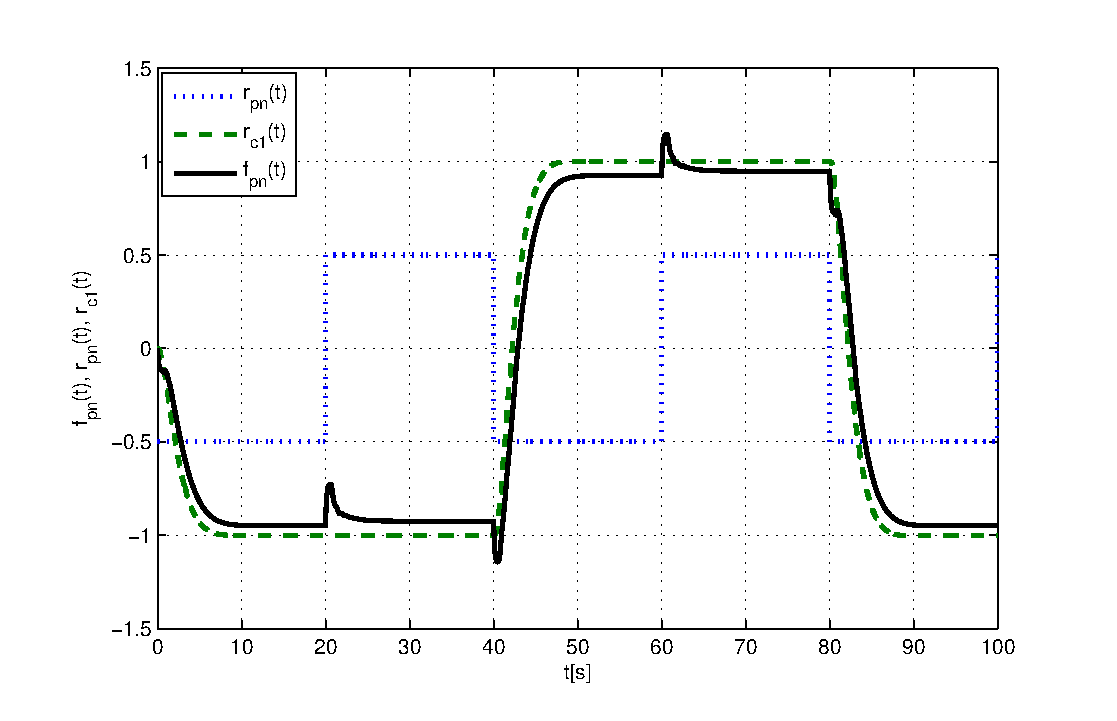
\includegraphics[width=3.5in]{figures/fault_detection_off_degrade}
  \caption{System response when using the {\em resilient power
    junction} under Assumption~\ref{A:resilient_pj} and integrator
  term of controller 4 is set to zero.}
  \label{fig:fault_detection_off_degrade}
\end{figure}
\begin{figure}
  \centering
  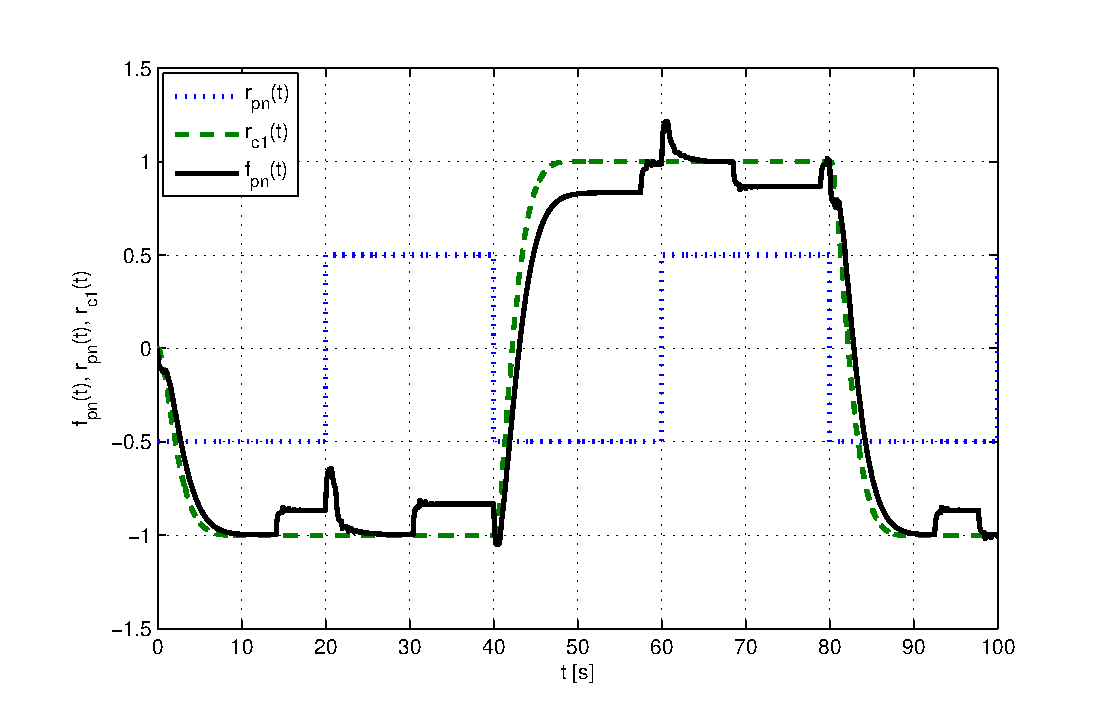
\includegraphics[width=3.5in]{figures/fault_detection_off_denial}
  \caption{System response when using the {\em resilient power
    junction} under Assumption~\ref{A:resilient_pj} and introducing a
    intermittent denial of service attack to controller 4.}
  \label{fig:fault_detection_off_denial}
\end{figure}
\begin{figure}
  \centering
  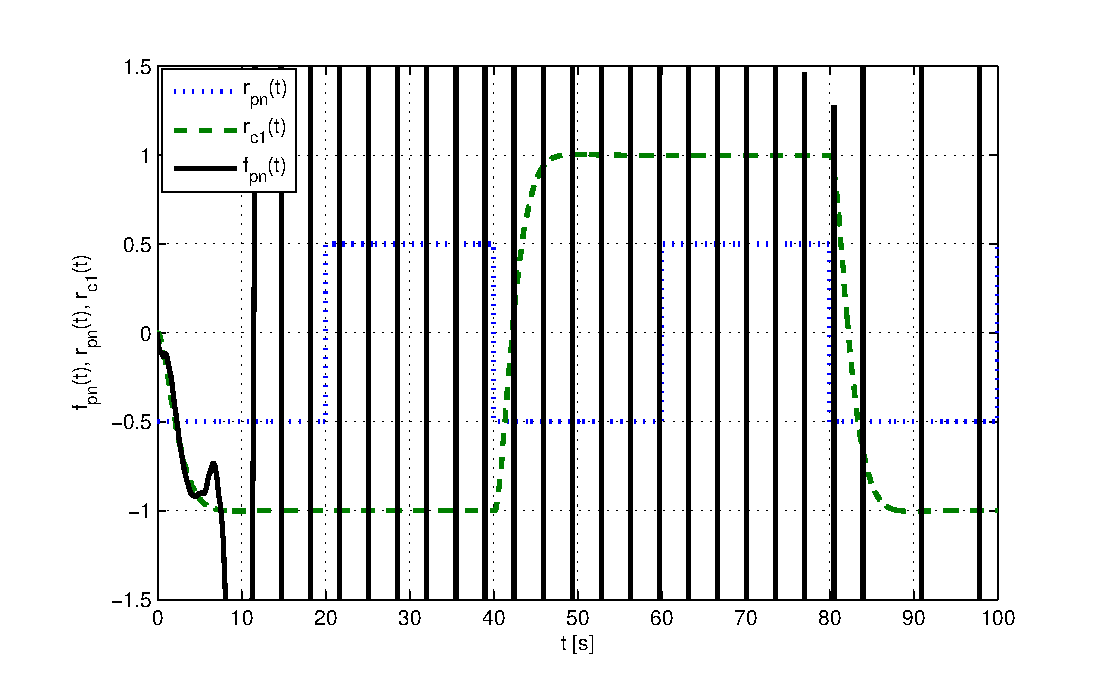
\includegraphics[width=3.5in]{figures/fault_detection_off}
  \caption{Unstable system response when using the {\em resilient power
    junction} under Assumption~\ref{A:resilient_pj} and introducing a
    highly unstable (and non-passive) digital-controller to the network.}
  \label{fig:fault_detection_off}
\end{figure}
\begin{figure}
  \centering
  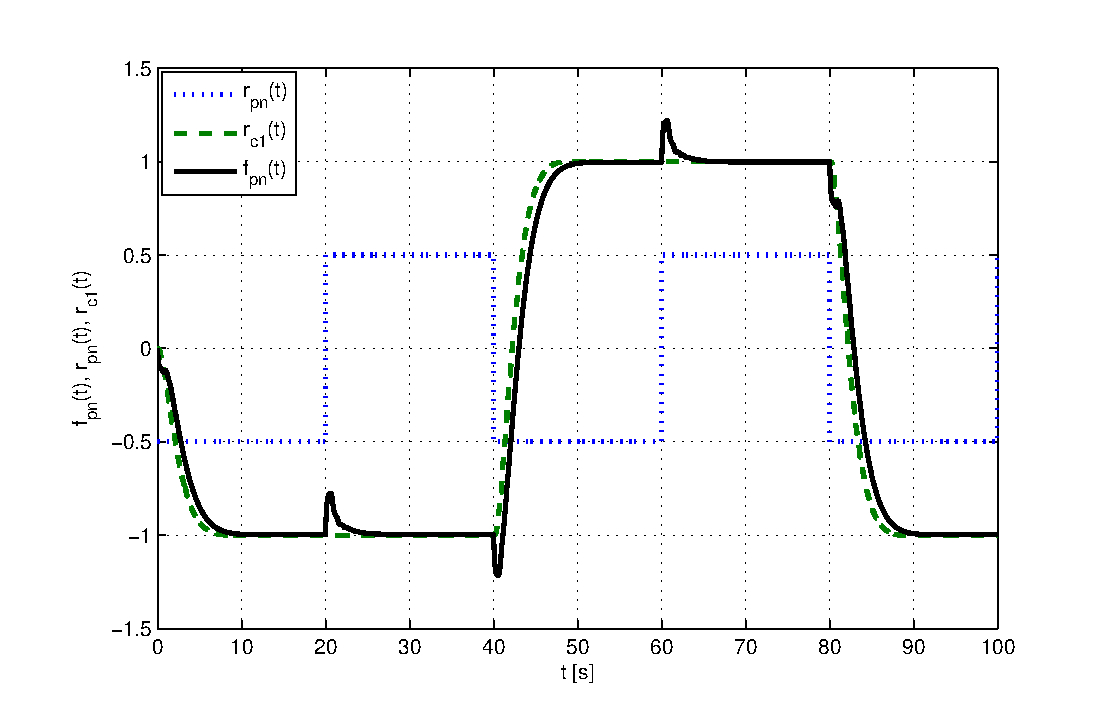
\includegraphics[width=3.5in]{figures/fault_detection_on}
  \caption{Stable system response when using the {\em resilient power
      junction} under Assumption~\ref{A:resilient_pj_ii}.}
  \label{fig:fault_detection_on}
\end{figure}
